\documentclass[12pt]{article}

% Espacement automatique apr�s certaines macros
\usepackage{xspace}

% Pour avoir des font presque T1 (EC?)... Meilleur output pdf.
%\usepackage[T1]{fontenc}
\usepackage{ae}
\usepackage{aecompl}
\usepackage{aeguill}

% Choses pratiques
\usepackage{graphicx}
\usepackage{subfigure}

\title{FreeWRL collision detection algorithmic overview}
\author{Nicolas Coderre\\CRC Canada}
% D�but du document %%%%%%%%%%%%%%%%%%%%%%%%%%%%%%%%%%%%%%%%
\begin{document}
\maketitle
\begin{abstract}
The collision algorithm used is a static interference test.
This test also returns the direction and displacement needed to eliminate the intersection.
In the case of displacements in the direction of the normal of the contact plane, It roughly calulates the geometric
intersection of the avatar and the half-prism of the polygon on the contact plane (polygon extendend to infinity in it's backface).
In the other case the displacements are made in the direction of the closest point (polyrep disp algo.)

This document explains the basic workings of the most important algorithms used.
It is assumed that the reader will be courageous enough to look at the source code. (or at least it's comments)
\end{abstract}

\section{Avatar representation}
A cylinder aligned on the up vector is used in most cases.
Another cylinder the height of ``step'' is appended for stepping.

With the IndexedFaceSet and Extrusion tests, the algorithm used is the new one.
Therefore, a sphere is used for the most part.
But a cylinder the height of ``step'' is still present for stepping.
It is not neccessarily in contact with the sphere. This causes a few stange behaviours.

\subsection{The basic piece of the puzzle : the polygon-cylinder intersection algorithm}
The algorithm roughly uses calculates the geometric intersection of the cylinder and
the polygon half-prism. By polygon half-prism I mean the space traversed by the
polygon it were sweeped in the oposite direction of it's normal.

It gets the points of the intersection, and minimises the projection of these points
on the normal vector. (takes the farthest point from the triangle's plane)
\begin{figure}[htb]
\centering
	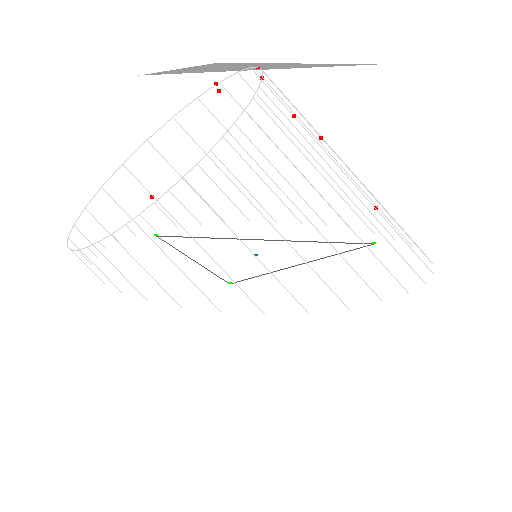
\includegraphics[angle=0,width=0.5\textwidth]{triangle_disp_points_triangle_plan}
	\label{figure:tridispplan}
\caption{Cylinder in triangle plane. Highest point is answer}
\end{figure}
\emph{(fig \ref{figure:tridispplan})}

\subsection{The bastard basic piece of the puzzle : the polygon-sphere intersection algorithm}
This one is used in the IndexedFaceSet and Extrusion tests.

The algorithm calculates the closest point of the polygon to the origin.
It then returns a vector in the direction of the closest point.
It's size is the difference between the distance to the closest point and the sphere radius.
(The displacement needed to put the point back on the surface)

\subsection{Stepping : the polygon-cylinder intersection algorithm}
The polygon-cylinder intersection algorithm has a variant that displaces only vertically.
It is used at pretty much random places inside the code to get the stepping effect.
It should be used more consitently. The way it is right now creates a few ugly jumping cases.

\subsection{Box displacement}

The algorithm uses the polygon-cylinder intersection algorithm on the faces frontfacing the avatar.
It then takes the minimum. This works flawlessly.
\begin{figure}[htb]
%\centering
	\subfigure[Delta z-.8361 ] {
		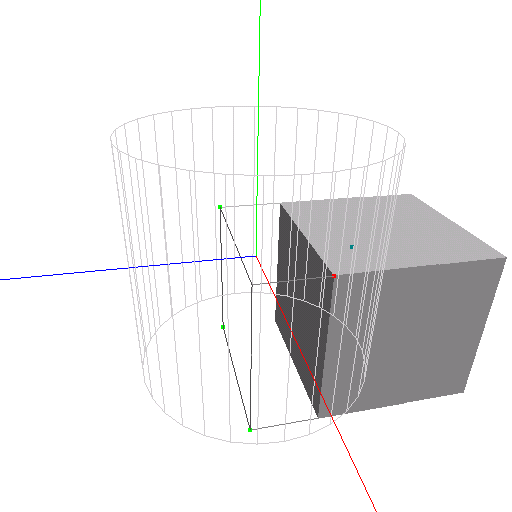
\includegraphics[angle=0,width=0.5\textwidth]{box_disp_side_1}
		\label{figure:boxdisp:a}
	}
	\subfigure[Delta x-.5686] {
		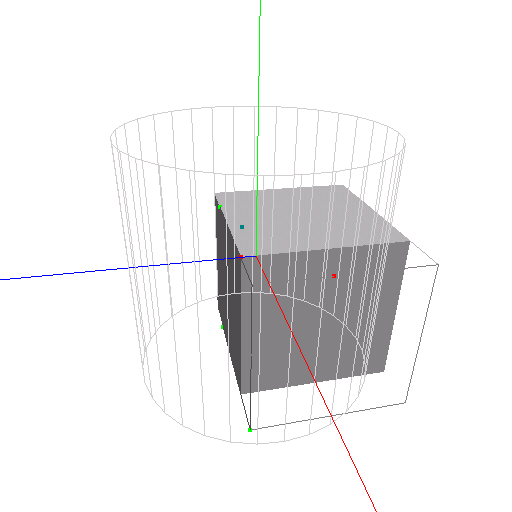
\includegraphics[angle=0,width=0.5\textwidth]{box_disp_side_2}
		\label{figure:boxdisp:b}
	}
	\subfigure[Delta y-.4525] {
		\includegraphics[angle=0,width=0.5\textwidth]{box_disp_side_3}
		\label{figure:boxdisp:c}
	}
\caption{Contribution of each face to the displacement. The minimum is chosen.}
\label{figure:boxdisp}
\end{figure}
\emph{(fig \ref{figure:boxdisp})}

The stepping code can bring stange stuff, though.

\subsection{Cone and cylinder}

This algorithm uses a hack.
It assumes the contact point will be on the plane passing through the origin and the cone/cylinder's axis.
Most of the time, this is the case, but not always. Still, the method gives excellent results.

The idea is to use a degenerated version of the polygon-cylinder algorithm, for lines and points.
The intersection tests are done on the lines of the surface that are on the forementionned plane.
\begin{figure}[htb]
%\centering
	\subfigure[] {
		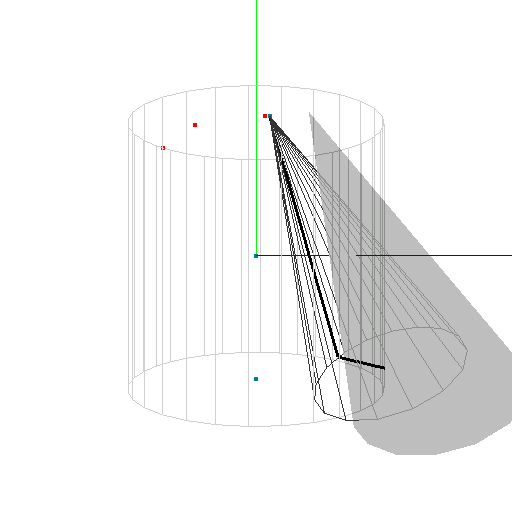
\includegraphics[angle=0,width=0.5\textwidth]{cone_disp}
		\label{figure:conicdisp:a}
	}
	\subfigure[] {
		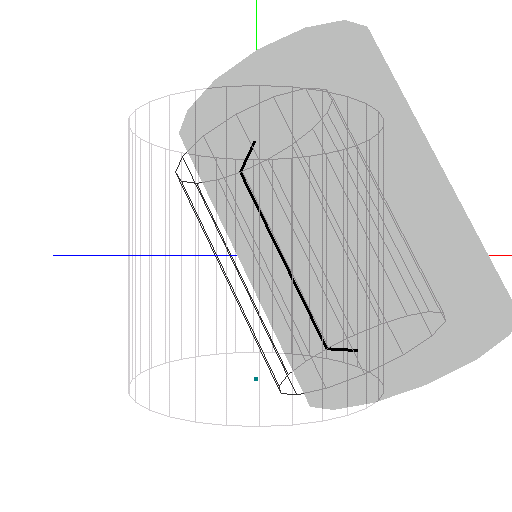
\includegraphics[angle=0,width=0.5\textwidth]{cylinder_disp}
		\label{figure:conicdisp:b}
	}
\caption{Intesection and displacement of cone and cylinder. In bold, the semgents used for calculation.}
\label{figure:conicdisp}
\end{figure}
\emph{(fig \ref{figure:conicdisp})}

The cone's top is represented by a point, with the normal upwards. It made more sense to clip that point
with a different normal than the side.

\subsection{Polyreps : IndexedFaceSets and Extrusions}

The algorithm uses the sphere intersection code. It is applied recursively to correct cases of concavity and coplanar sufaces.
\begin{figure}[htb]
%\centering
	\subfigure[One polygon's displacement changes the intersection case of the other.] {
		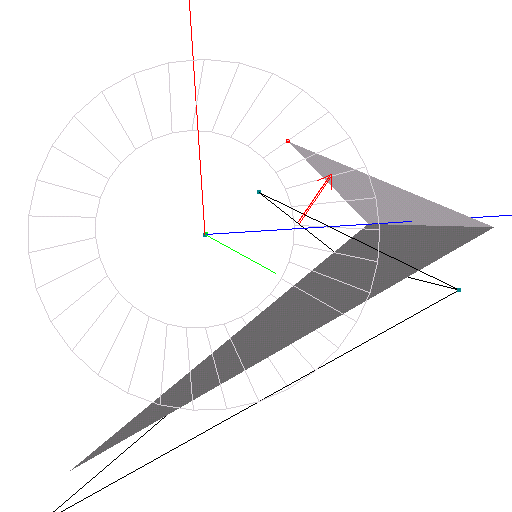
\includegraphics[angle=0,width=0.5\textwidth]{polydisp_concave_arrow}
		\label{figure:polydisp:concave}
	}
	\subfigure[We must not chose the minimum displacement in the case of coplanar sufaces.] {
		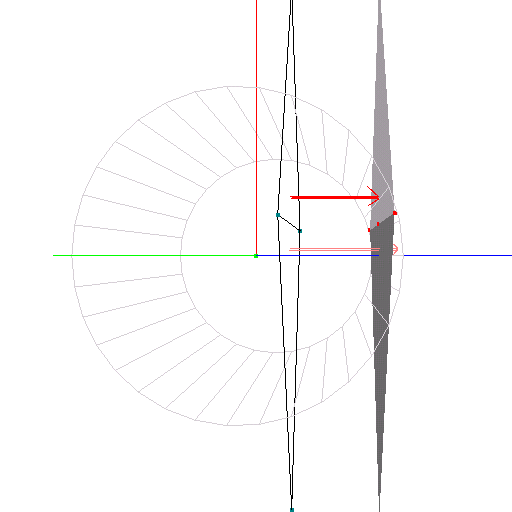
\includegraphics[angle=0,width=0.5\textwidth]{polydisp_parallel_arrow}
		\label{figure:polydisp:parallel}
	}
\caption{Situations fixed by recursivly calling the polyrep-disp algorithm.}
\label{figure:polydisp}
\end{figure}
\emph{(fig \ref{figure:polydisp})}

For doublesided polyreps, it reverses the normal when the poly is backfacing. One exception: after one
pass, either we are frontfacing or backfacing. This way, one pass won't ambigusly choose to
go on a different side of a surface then previous calculations.

Stepping value is calculated simultaneously. The stepping result is used, unless
the sphere intersects with the polyrep. The normal displacement code has priority.

\subsection{Polyreps : Text}

This algorithm could use the sphere intersection code. But it works great with the cylinder algorithm.

It optimizes by keeping the same normal all the way through, and uses the maximum displacement
instead of the minimum, because the faces are coplanar. \emph{(fig \ref{figure:polydisp:parallel})}

\subsection{Polyreps : ElevationGrid}

This algorithm uses the pregenerated points in the polyrep structure instead of recalculating them.
It does optimization to only check the quads inside a probable region.
The optimization depends on the special organisation of the triangles in the polyrep structure.
If the genpolyrep function changes, this code must be changed too.

The probable region is calculated by projecting the cylinder's enclosing sphere on the
grid's plane. This gives two coordinate ranges (x and z).
Tranformations and intersections are only calculated on those points/faces.

\end{document}




